\documentclass[ST]{subfiles}

\begin{document}
\begin{figure}
\centering
\begin{tabular}{cc}
  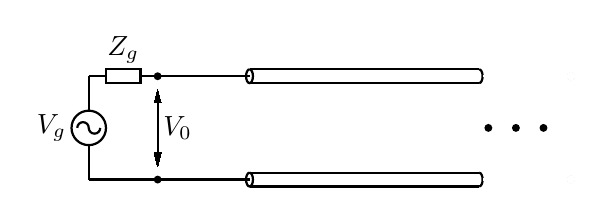
\begin{tikzpicture}[scale=1.75]
% dpic version 2010.11.28 option -g for TikZ and PGF 1.01
\ifx\dpiclw\undefined\newdimen\dpiclw\fi
\global\def\dpicdraw{\draw[line width=\dpiclw]}
\global\def\dpicstop{;}
\dpiclw=0.8bp
\dpiclw=0.8bp
\dpicdraw (0,0)
 --(0,0.25)\dpicstop
\dpicdraw (0,0.375) circle (0.049213in)\dpicstop
\dpicdraw (-0.083333,0.375)
 ..controls (-0.083333,0.398012) and (-0.064679,0.416667)
 ..(-0.041667,0.416667)
 ..controls (-0.018655,0.416667) and (0,0.398012)
 ..(0,0.375)\dpicstop
\dpicdraw (0,0.375)
 ..controls (0,0.351988) and (0.018655,0.333333)
 ..(0.041667,0.333333)
 ..controls (0.064679,0.333333) and (0.083333,0.351988)
 ..(0.083333,0.375)\dpicstop
\dpicdraw (0,0.5)
 --(0,0.75)\dpicstop
\draw (-0.125,0.375) node[left=-1.5bp]{$ V_g$};
\dpicdraw (0,0.75)
 --(0.125,0.75)\dpicstop
\dpicdraw (0.375,0.75)
 --(0.375,0.8)
 --(0.125,0.8)
 --(0.125,0.7)
 --(0.375,0.7)
 --(0.375,0.75)\dpicstop
\dpicdraw (0.375,0.75)
 --(0.5,0.75)\dpicstop
\draw (0.25,0.8) node[above=-1.5bp]{$ Z_g$};
\dpicdraw[fill=black](0.5,0.75) circle (0.007874in)\dpicstop
\dpicdraw[fill=black](0.5,0) circle (0.007874in)\dpicstop
\filldraw[line width=0bp](0.525,0.55625)
 --(0.5,0.65625)
 --(0.475,0.55625) --cycle
\dpicstop
\dpicdraw (0.5,0.633344)
 --(0.5,0.19375)\dpicstop
\filldraw[line width=0bp](0.475,0.19375)
 --(0.5,0.09375)
 --(0.525,0.19375) --cycle
\dpicstop
\draw (0.5,0.375) node[right=-1.5bp]{$V_0$};
\dpicdraw (2.858333,0.75)
 --(3.5,0.75)\dpicstop
\dpicdraw (0.5,0.75)
 --(1.166667,0.75)\dpicstop
\dpicdraw (1.166667,0.7)
 --(2.833333,0.7)\dpicstop
\dpicdraw (2.833333,0.7)
 ..controls (2.847141,0.7) and (2.858333,0.722385)
 ..(2.858333,0.75)
 ..controls (2.858333,0.777615) and (2.847141,0.8)
 ..(2.833333,0.8)\dpicstop
\dpicdraw (2.833333,0.8)
 --(1.166667,0.8)\dpicstop
\dpicdraw (1.166667,0.8)
 ..controls (1.152859,0.8) and (1.141667,0.777615)
 ..(1.141667,0.75)
 ..controls (1.141667,0.722385) and (1.152859,0.7)
 ..(1.166667,0.7)
 ..controls (1.180474,0.7) and (1.191667,0.722385)
 ..(1.191667,0.75)
 ..controls (1.191667,0.777615) and (1.180474,0.8)
 ..(1.166667,0.8)\dpicstop
\dpicdraw[fill=black](3.5,0.75) circle (0.007874in)\dpicstop
\dpicdraw[fill=black](3.5,0) circle (0.007874in)\dpicstop
\dpicdraw (2.858333,0)
 --(3.5,0)\dpicstop
\dpicdraw (0.5,0)
 --(1.166667,0)\dpicstop
\dpicdraw (1.166667,-0.05)
 --(2.833333,-0.05)\dpicstop
\dpicdraw (2.833333,-0.05)
 ..controls (2.847141,-0.05) and (2.858333,-0.027615)
 ..(2.858333,0)
 ..controls (2.858333,0.027615) and (2.847141,0.05)
 ..(2.833333,0.05)\dpicstop
\dpicdraw (2.833333,0.05)
 --(1.166667,0.05)\dpicstop
\dpicdraw (1.166667,0.05)
 ..controls (1.152859,0.05) and (1.141667,0.027615)
 ..(1.141667,0)
 ..controls (1.141667,-0.027615) and (1.152859,-0.05)
 ..(1.166667,-0.05)
 ..controls (1.180474,-0.05) and (1.191667,-0.027615)
 ..(1.191667,0)
 ..controls (1.191667,0.027615) and (1.180474,0.05)
 ..(1.166667,0.05)\dpicstop
\dpicdraw (0.5,0)
 --(0,0)\dpicstop
\dpicdraw[fill=black](3.3,0.375) circle (0.007874in)\dpicstop
\dpicdraw[fill=black](3.1,0.375) circle (0.007874in)\dpicstop
\dpicdraw[fill=black](2.9,0.375) circle (0.007874in)\dpicstop
\draw[thick,white] (2.864,0)--(3.5,0);
\draw[thick,white] (2.864,0.75)--(3.5,0.75);
\draw[fill=white, color=white] (3.5,0.75) circle (0.8pt);
\draw[fill=white, color=white] (3.5,0) circle (0.8pt);
\end{tikzpicture}
 &
 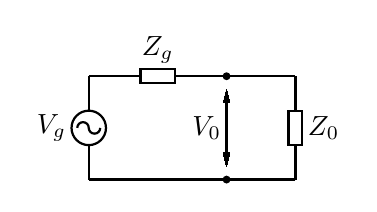
\begin{tikzpicture}[scale=1.75]
% dpic version 2010.11.28 option -g for TikZ and PGF 1.01
\ifx\dpiclw\undefined\newdimen\dpiclw\fi
\global\def\dpicdraw{\draw[line width=\dpiclw]}
\global\def\dpicstop{;}
\dpiclw=0.8bp
\dpiclw=0.8bp
\dpicdraw (0,0)
 --(0,0.25)\dpicstop
\dpicdraw (0,0.375) circle (0.049213in)\dpicstop
\dpicdraw (-0.083333,0.375)
 ..controls (-0.083333,0.398012) and (-0.064679,0.416667)
 ..(-0.041667,0.416667)
 ..controls (-0.018655,0.416667) and (0,0.398012)
 ..(0,0.375)\dpicstop
\dpicdraw (0,0.375)
 ..controls (0,0.351988) and (0.018655,0.333333)
 ..(0.041667,0.333333)
 ..controls (0.064679,0.333333) and (0.083333,0.351988)
 ..(0.083333,0.375)\dpicstop
\dpicdraw (0,0.5)
 --(0,0.75)\dpicstop
\draw (-0.125,0.375) node[left=-1.5bp]{$ V_g$};
\dpicdraw (0,0.75)
 --(0.375,0.75)\dpicstop
\dpicdraw (0.625,0.75)
 --(0.625,0.8)
 --(0.375,0.8)
 --(0.375,0.7)
 --(0.625,0.7)
 --(0.625,0.75)\dpicstop
\dpicdraw (0.625,0.75)
 --(1,0.75)\dpicstop
\draw (0.5,0.8) node[above=-1.5bp]{$ Z_g$};
\dpicdraw[fill=black](1,0.75) circle (0.007874in)\dpicstop
\dpicdraw[fill=black](1,0) circle (0.007874in)\dpicstop
\filldraw[line width=0bp](1.025,0.55625)
 --(1,0.65625)
 --(0.975,0.55625) --cycle
\dpicstop
\dpicdraw (1,0.633344)
 --(1,0.19375)\dpicstop
\filldraw[line width=0bp](0.975,0.19375)
 --(1,0.09375)
 --(1.025,0.19375) --cycle
\dpicstop
\draw (1,0.375) node[left=-1.5bp]{$V_0$};
\dpicdraw (1,0.75)
 --(1.5,0.75)\dpicstop
\dpicdraw (1.5,0.75)
 --(1.5,0.5)\dpicstop
\dpicdraw (1.5,0.25)
 --(1.55,0.25)
 --(1.55,0.5)
 --(1.45,0.5)
 --(1.45,0.25)
 --(1.5,0.25)\dpicstop
\dpicdraw (1.5,0.25)
 --(1.5,0)\dpicstop
\draw (1.55,0.375) node[right=-1.5bp]{$ Z_0$};
\dpicdraw (1.5,0)
 --(1,0)\dpicstop
\dpicdraw (1,0)
 --(0,0)\dpicstop
\end{tikzpicture}\\
  $(a)$&$(b)$
\end{tabular}
 \caption{L�nea de transmisi�n infinita sin p�rdidas en $(a)$ y su circuito equivalente en $(b)$}
 \label{fig:LTxInfSinPerMasCtoEquBajFre}
 \end{figure}
\end{document}

